This section illustrates how the system will be implemented and tested.

\subsection{Implementation Plan}

All components will be implemented and tested using a bottom-up approach. Development will begin with the components at the lower levels of the hierarchy, with each component tested using drivers to simulate interactions with components that are not yet developed.

As each component is completed, it will be integrated into the system, replacing any drivers that previously simulated its behavior.

By scaling up incrementally from a smaller subset of the system (divide and conquer), this method simplifies error tracking and debugging.

\subsection{Features identification}
\begin{listoffeatures}{F}

    \item \textbf{Recommendations}
    This core feature provides personalized recommendations to students and company members based on their interests.  
    Given its importance, this will be the first feature to be developed and tested.

    \item \textbf{Login and Registration}
    These features allow users to access the platform.  
    As the initial point of entry to the system and a potential point of vulnerability, they require rigorous and early testing.  
    For this reason, they will be the second feature to be implemented and tested.

    \item \textbf{Upload CVs}
    This feature enables students to add, modify, and delete their uploaded CVs, providing guidance and suggestions throughout the process.

    \item \textbf{Upload and Search for Internship proposals} 
    This feature functions similarly to \textit{Upload CVs}, enabling company members to add, modify, and delete internship proposals.  
    Additionally, it provides students with the ability to search for available internships.
    
    \item \textbf{Matching proposals}.
    This feature facilitates interactions between students and company members by allowing them to send match proposals, indicating mutual interest on the platform.

    \item \textbf{Conduct interviews}.
    This feature supports companies in conducting interviews by enabling the creation of a chat between students and company members.  
    It also schedules interviews and allows students to accept or decline offers.

    \item \textbf{Monitor interviews}.
    This feature consolidates functionalities for monitoring internships, helping all parties involved to address and resolve any issues that may arise.
\end{listoffeatures}

\subsection{Commponent Integration and Testing}

\compDevel{Recommendations}{
The first components to be developed and tested will be the Data Manager and the Recommendation Manager.
}{0.3}

\compDevel{Login and Registration}{
The next components to be integrated will be the Registration Manager, the Login Manager and the Email Manager. 
The first two must be tested accurately to keep the system safe from malicious input.
}{0.3}


\compDevel{Upload CVs}{
The next comonents two be developed will be the CV Manager and the Suggestion Manager.
}{0.3}

\compDevel{Upload and search for internship proposals}{
The next component to be developed will be the Internship Proposal Manager.
}{0.3}

\compDevel{Matching Proposals}{
The components that will be developed are the the Matching Proposal and the Notify Manager.
}{0.3}

\compDevel{Conduct interviews}{
The next component will be the Selection Manager, the Interview Scheduler and the Chat Manager.
}{0.2}

\compDevel{Monitor interviews}{
The component that will be developed is the Internship Status Manager.
}{0.2}

%Finally the last componennt, the controller will be developed.
%
%\begin{figure}[H]
%    \centering
%    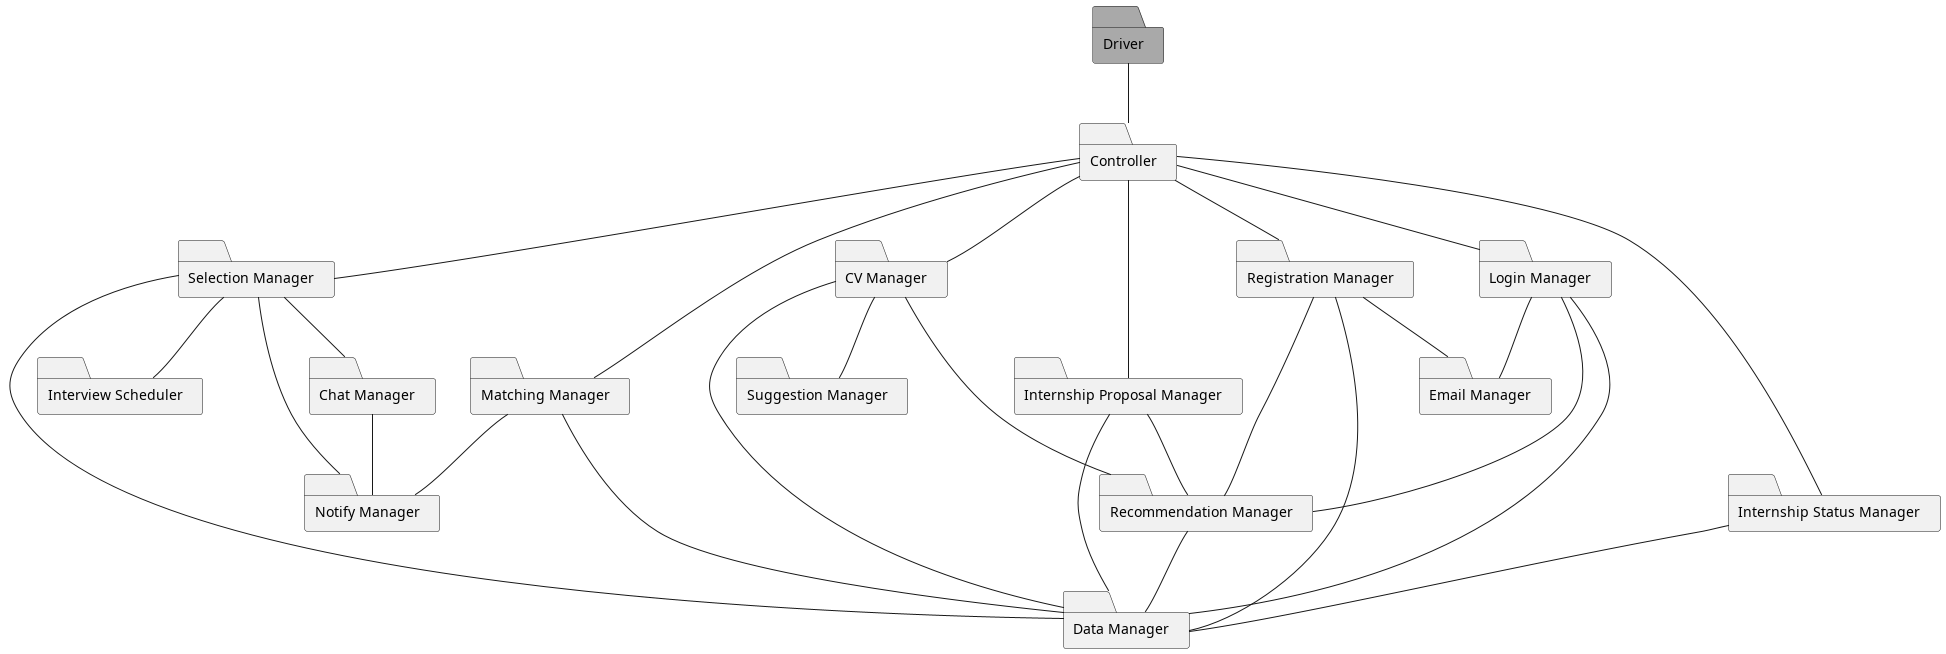
\includegraphics[scale=0.2]{Implementation_integration_and_test_plan/uml_diagrams/feat8.png}
%    \caption{Login and registration developement.}
%\end{figure}

\subsection{System Testing}
The system must be tested to verify that each functional and non-functional requirement as stated in the RASD document is respected. To do so, the following steps will be followed

\begin{itemize}
    \item \textbf{Functional Testing} Functional testing will verify that all requirements specified in the RASD document are correctly implemented and adhered to.  
    
    \item \textbf{Performance Testing} The system's ability to handle the expected number of requests will be evaluated to ensure it operates within the performance parameters defined in the RASD document.  
    
    \item \textbf{Load Testing} The system will be subjected to increasing levels of load up to its breakpoint to identify vulnerabilities, such as security issues that could lead to data leaks of users' information.  
    
    \item \textbf{Stress Testing} Stress testing will simulate scenarios where the system exceeds its breakpoint, such as handling a high number of concurrent requests or operating with reduced resources, to assess how quickly and effectively it recovers from failure.  
    
    \item \textbf{User Interface Testing.} The system's interface will be tested across a wide range of web browsers to ensure it functions properly and delivers a consistent user experience.
\end{itemize}

\newpage